\documentclass[letterpaper, 10pt]{article}
\usepackage[top = 3cm, bottom = 3cm, left = 2.5cm, right = 2.5cm]{geometry}


\title{Simulation of partially clonal diploid populations with simuPOP v.1.0.8}
\author{Zhian N. Kamvar}
\date{\today}
\newcommand{\tab}{\hspace*{1.5em}}
\usepackage{mathtools, setspace, lineno}
\usepackage[pdftex, dvipdfm, dvips]{graphicx}
\usepackage[utf8]{inputenc}


\begin{document}
\maketitle
\linenumbers
\setstretch{2}
\section{Methods}
\tab All simulations were performed via the python scripted, individual-based simulation program SimuPOP (v.1.0.8) under ten different rates of sexual reproduction (0\%, 0.01\%, 0.05\%, 0.1\%, 1\%, 5\%, 10\%, 20\%, 50\%, and 100\%).
These rates correspond to the proportion of offspring that would be produced via sexual reproduction. 
Each simulation consisted of a single heterothallic, isolated population that contained a fixed census size of 10,000 individuals with 10 loci that had 6 to 10 alleles at each locus with variable frequencies. 

To avoid stochastic variation among rates of sexual reproduction, 100 unique seed populations were initialized with the parameters listed above.
Diploid individuals were assigned genotypes at all loci and then underwent a `burn in' period of random mating for 1,000 generations to bring the population to equilibrium. 
For each level of sexual reproduction, the seed populations were run under the specified mating scheme for 10,000 generations with a mutation rate of $1E^{-5}$ applied to parental individuals over all loci each generation before mating. 
Cloned offspring were simply copied from the $F1$ to the $F2$ generation, whereas those derived from sexual reproduction were produced from the combination of two parents. 
Both operations were performed using random sampling with replacement from the $F1$ generation.
Populations were saved after every 1,000 generations and 10 sub samples of four sizes (10, 25, 50, and 100 individuals) were randomly drawn and saved in FSTAT format. There were 40,000 data sets in total, resulting in 160,000 values of $I_A$ and $\bar{r}_d$ analyzed.

Statistical analysis was performed using the R package \textit{poppr} (v.1.0.0). 
The summary statistics $I_A$ and $\bar{r}_d$ were calculated and their respective p-values were determined via permutation analysis\footnote{
Four different methods of permutation were utilized.
The first method was a method of permutation developed by Agapow and Burt in the program \textit{multilocus}.
This method would reshuffle genotypes at each locus in order to simulate the null hypothesis of unlinked loci. 
The second method was a method of permutation that would shuffle the alleles at each locus to simulate sexual reproduction within the observed population.
The third and fourth methods were parametric and non-parametric bootstrapping of alleles at each locus, or sampling with replacement. 
For the parametric method, at each locus, observed allele frequencies were calculated and then resampled at those frequencies to reconstruct the locus. 
The non-parametric method would simply resample alleles at each locus with replacement, regardless of frequency.
Both of the bootstrap methods would simulate the null hypothesis of sexual reproduction from a larger population.}. Regarding a test of the resampling methods, ROC curves were created using the data with a sex rate of 1 to represent the null compared against all other rates of sexual reproduction with values of alpha at intervals of 0.001. The area under the ROC curve (AUC) was calculated using the \texttt{trapz} function in the \textit{caTools} package. Since the data was non normal, the Kruskal-Wallis test was calculated using Base R and all graphics were created with the \textit{ggplot2} package.

\section{Results}
\tab 
Table 1. Kruskal-Wallis test comparison.
% latex table generated in R 3.0.1 by xtable 1.7-1 package
% Fri Jun 28 16:23:49 2013
\begin{table}[ht]
\centering
\begin{tabular}{rcc}
  \hline
Comparison & With Non-Parametric Bootstrap & Without Non-Parametric Bootstrap \\ 
  \hline
AUC for $I_A$ & 0.93997 & 0.92008 \\ 
  AUC for $\bar{r}_d$ & 0.97545 & 0.97234 \\
  \hline
  True Positive $I_A$ & 0.00000 & 0.00000 \\ 
  True Positive $\bar{r}_d$ & 0.00402 & 0.78424 \\
  \hline  
  False Positive $I_A$ & 0.00432 & 0.35469 \\ 
  False Positive $\bar{r}_d$ & 0.00181 & 0.30023 \\  
  \hline
  p-value $I_A$ & 0.00004 & 0.90869 \\ 
  p-value $\bar{r}_d$ & 0.00001 & 0.90699 \\ 
   \hline
\end{tabular}
\end{table}


The first set of charts represent all finite values of the data set:

\begin{center}
Figure 1a.\\
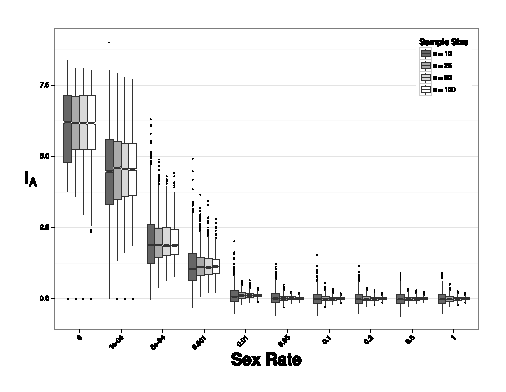
\includegraphics{figures/Ia_chart.eps}\\Figure 1b.\\
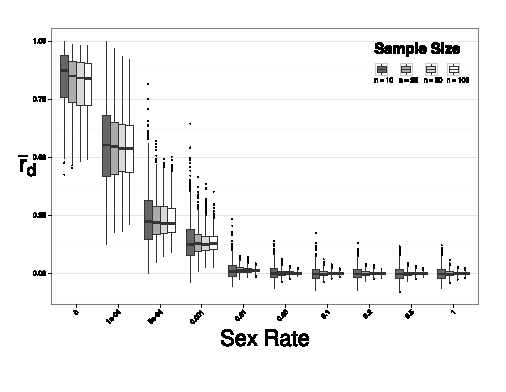
\includegraphics{figures/rbarD_chart.eps}\\Figure 1c.\\
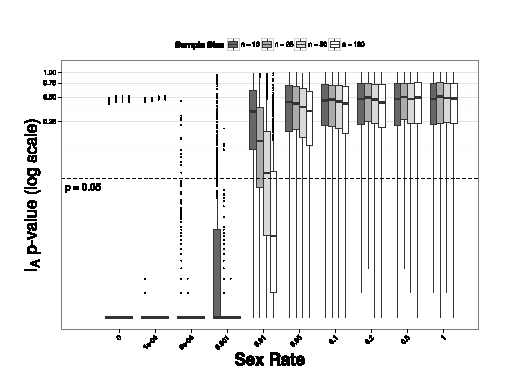
\includegraphics{figures/Ia_pval.eps}\\Figure 1d.\\
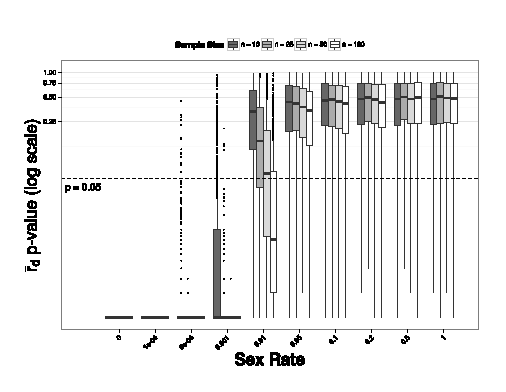
\includegraphics{figures/rbarD_pval.eps}\\
\end{center}

The second set represent the data sets with missing values of $\bar{r}_d$ removed.

\begin{center}
Figure 2a.\\
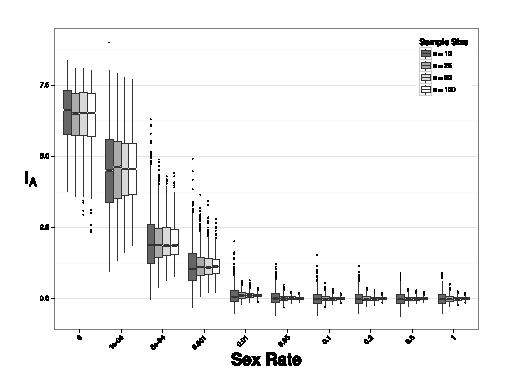
\includegraphics{figures/Ia_chart2.eps}\\Figure 2b.\\
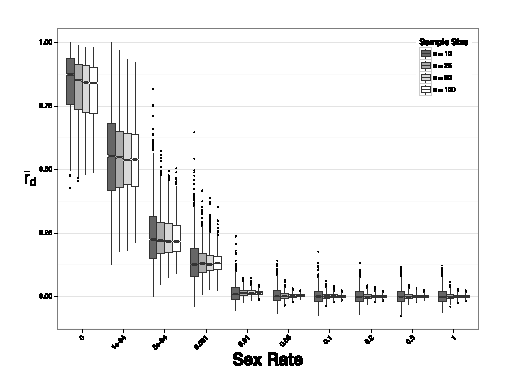
\includegraphics{figures/rbarD_chart2.eps}\\Figure 2c.\\
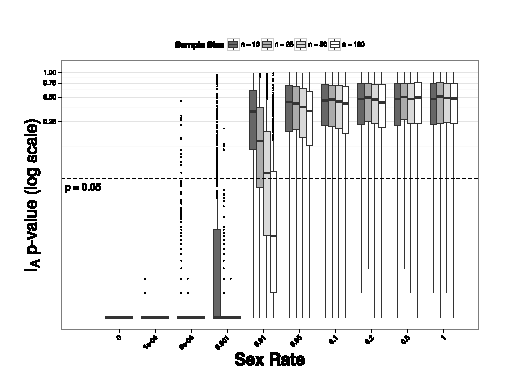
\includegraphics{figures/Ia_pval2.eps}\\Figure 2d.\\
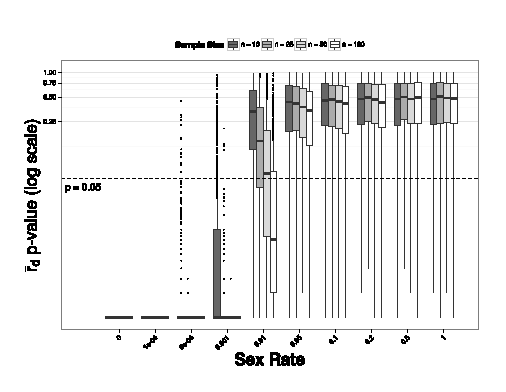
\includegraphics{figures/rbarD_pval2.eps}\\
\end{center}

\end{document}
